\subsubsection{Controller}
\lable{sec:Controller}
	Die Controller-Hardware steuert die Motoren der Ballzuführung, der Stepper für die Ausrichtung der Apparatur und die Motoren zur Beschleunigung der Bälle. Sobald der Controller das Startsignal vom Master erhält, wird dieser den Motor zur Ballbeschleunigung aktivieren und hoch drehen lassen. Weiter erhält der Controller vom Master die Angabe, in welchem Winkel sich der Korb befindet. Anhand dieser wird die benötigten Schritte berechnen und die resultierenden Befehle an die Motorsteuerung absetzen. Sobald die Apparatur die richtige Ausrichtung eingenommen hat, wird die Ballzuführung aktiviert, um die Bälle in den Korb zu befördern. Mittels eines kleinen Sensors werden die Bälle gezählt und wenn der letzte Ball abgefeuert wurde, wird dies dem Master signalisiert.\\
	\begin{wrapfigure}{r}{0.45\textwidth}
		\centering
		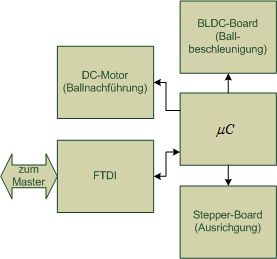
\includegraphics[width=0.44\textwidth]{Enddokumentation/Loesungskonzept/Bilder/Blockschaltbild_Controller.png}
		\caption{Blockschaltbild der Controller-Hardware}
		\label{fig:Blockschaltbild_Controller}
	\end{wrapfigure}
	Die Abbildung \ref{fig:Blockschaltbild_Controller} zeigt auf, wie die Controller-Hardware aufgebaut sein wird. Die BLDC- und Stepper-Ansteuerung wird auf separaten Boards realisiert, wobei die Stepper-Hardware durch die PREN-ET
	entwickelt und in dieser Gruppe eingesetzt wird. Als Schnittstelle zwischen den Boards und dem Controller wird SPI eingesetzt, da ein Hauptchip der Stepper-Ansteuerung nur über SPI angesprochen werden kann. Die Kommunikation mit dem Master wir über UART stattfinden, das über den FTDI-Chip auf USB emuliert wird. Die Ansteuerung des DC-Motors wird mittels PWM realisiert.